\documentclass{jib}
\newlength{\platz}
\setlength{\platz}{15pt}
\RequirePackage{listings}
\lstset{%
  basicstyle=\ttfamily,
  fontadjust,
  flexiblecolumns=true,
  frame=L,
  xleftmargin=15pt,
  framesep=5pt,
  emphstyle=\rmfamily\itshape}

\usepackage{pdfpages}

%%%%%%%%%%%%%%%%%%%%%%%%%%%%%%%%%%%%%%%%%%%%%%%%%%%%%%%%%%
% JIB Header/Footer
%%%%%%%%%%%%%%%%%%%%%%%%%%%%%%%%%%%%%%%%%%%%%%%%%%%%%%%%%%
\jibvolume{XX} % insert volume
\jibissue{X}   % insert issue
\jibpages{XXX} % insert article ID
\jibyear{XXXX} % insert year
\makeHeaderFooter{} % leave as is
%%%%%%%%%%%%%%%%%%%%%%%%%%%%%%%%%%%%%%%%%%%%%%%%%%%%%%%%%%

\begin{document}

%%%%%%%%%%%%%%%%%%%%%%%%%%%%%%%%%%%%%%%%%%%%%%%%%%%%%%%%%%
%
% Title Page
%
%%%%%%%%%%%%%%%%%%%%%%%%%%%%%%%%%%%%%%%%%%%%%%%%%%%%%%%%%%

\begin{jibtitlepage}

\jibtitle{The Simulation Experiment Description Markup Language (SED-ML):\\
Language Specification for Level~1 Version~4}


% Please make sure to use unique footnote characters for each author
\jibauthor{%
  Matthias K{\"o}nig\iref{humboldt},
  Frank T. Bergmann\iref{heidelberg},
  Lucian P. Smith\iref{uw},
  Alan Garny\iref{auckland},
  David Nickerson\iref{auckland},
  Dagmar Waltemath\iref{greifswald},
  Thomas Helikar\iref{nebraska},
  Jonathan Karr\iref{sinai}
  Herbert Sauro\iref{uw}
}

%\addjibinstitution{imbio}{IMBio, Ralf Hofest\"adt, Bielefeld University, Faculty of Technology, Bioinformatics Department, D-33501 Bielefeld, Germany, \url{http://www.imbio.de}}
\addjibinstitution{humboldt}{Humboldt University Berlin, DE}
\addjibinstitution{heidelberg}{BioQUANT/COS, Heidelberg University, Germany}
\addjibinstitution{uw}{University of Washington, US}
\addjibinstitution{auckland}{Auckland Bioengineering Institute, New Zealand}
\addjibinstitution{greifswald}{University of Greifswald, Germany}
\addjibinstitution{nebraska}{University of Nebraska, USA}
\addjibinstitution{sinai}{Icahn School of Medicine at Mount Sinai, USA}

\end{jibtitlepage}


% adjusts the width of the abstract, please do not change!
%\begin{adjustwidth}{}{1cm} %LS NOTE:  'adjustwidth' not recognized in my setup.

\renewcommand{\baselinestretch}{1.0}
\abstract{
The increasing use of computational simulation experiments to inform modern biological research creates new challenges to annotate, archive, share and reproduce such experiments. The Minimum Information About a Simulation Experiment (MIASE) proposes a minimal set of information that should be provided to allow the reproduction of simulation experiments among users and software tools.

SED-ML encodes in a computer-readable exchange format the information required by MIASE to enable reproduction of simulation experiments. It has been developed as a community project and it is defined in a detailed technical specification and additionally provides an XML schema.

SED-ML Level~1 Version~4 covers the description of time course and steady state simulations, parameter estimation experiments, and introduces a generic construct to allow new experiments to be described without the need to update this core specification.  For all descriptions, SED-ML provides a way to define the data, models, modifications, simulations, analyses, and results of each experiment it describes.  These descriptions are independent of the underlying model implementation.  SED-ML is a software-independent format for encoding the description of simulation experiments; it is not specific to particular simulation tools.  Additional materials and resources are available from the SED-ML project website at \url{http://sed-ml.org/}.}

%\end{adjustwidth} % please do not change %LS NOTE:  'adjustwidth' not recognized in my setup.


% Include your PDF document
\clearpage
\setlength{\voffset}{0cm}
\setlength{\hoffset}{0cm}
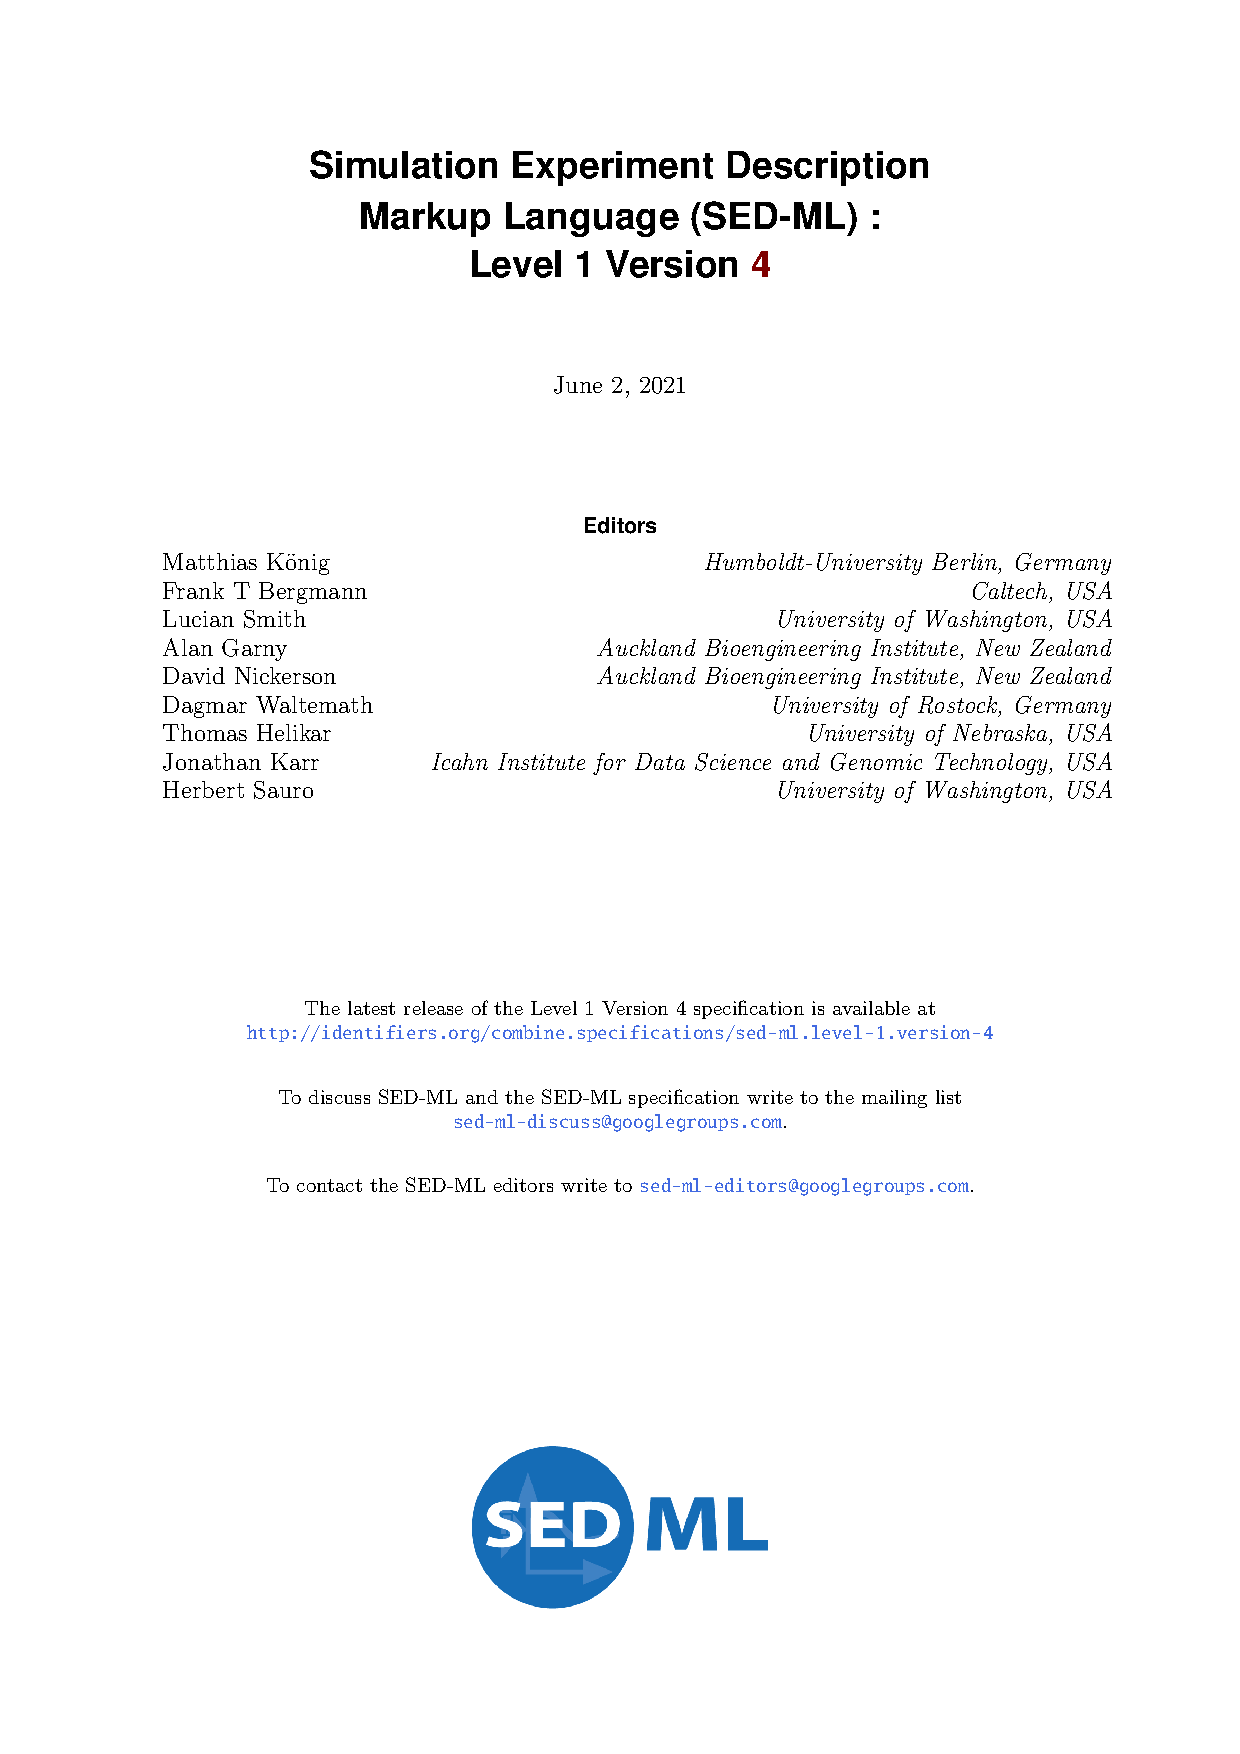
\includepdf[pages=-]{sed-ml-L1V4.pdf}

\end{document}
